%NOTE: COMPILE IN TERMINAL USING LUALATEX
\documentclass[a4paper,8pt]{standalone}

\usepackage{tikz-feynman}
%\usetikzlibrary{external}             %% Load the `external` library
%\tikzexternalize
%\immediate\write18{mkdir -p pgf-img}
%\tikzexternalize[                     %% Activate externalization
%  system call={                       %% Use lualatex in system call
%    lualatex \tikzexternalcheckshellescape -halt-on-error -interaction=batchmode -jobname="\image" "\texsource" || rm "\image.pdf"
%  },
%]

\begin{document}

%\feynmandiagram [horizontal=a to d]{
%    b -- [gluon] c -- [fermion,edge label'=$t$] c1 -- [gluon] b1,
%    c -- [fermion,edge label=$t$] a -- [fermion,edge label=$\bar t$] c1,
%    a -- [scalar,edge label=$H$] d,
%    b -- [opacity=0] b1,
%};

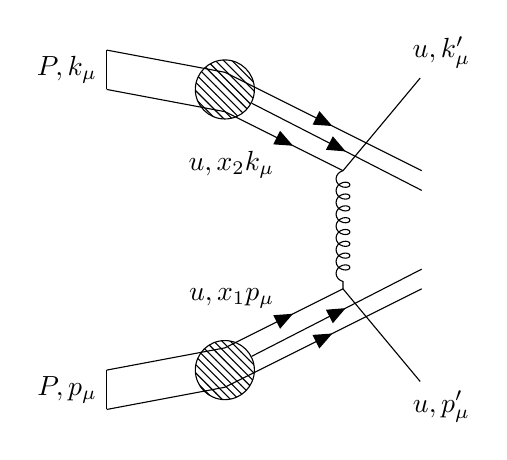
\begin{tikzpicture}
    \begin{feynman}
        \vertex (a1);
        \vertex[above=-0.1cm of a1,blob] (a2) {};
        \vertex[above=0.5cm of a1] (a3);
        \vertex[left=1.5cm of a2] (a4);
        \vertex[above=0.5cm of a4] (a5);

        \vertex[below=3cm of a1] (b1);
        \vertex[below=-0.1cm of b1,blob] (b2) {};
        \vertex[below=0.5cm of b1] (b3);
        \vertex[left=1.5cm of b2] (b4);
        \vertex[below=0.5cm of b4] (b5);

        \vertex at ($(a1)+(1.5cm,-0.75cm)$) (c1);
        \vertex at ($(c1)+(1cm,-0.25cm)$) (c2);
        \vertex[above=0.25cm of c2] (c3);

        \vertex[below=1.5cm of c1] (d1);
        \vertex at ($(d1)+(1cm,0.25cm)$) (d2);
        \vertex[below=0.25cm of d2] (d3);

        \vertex at ($(c3)+(0.25cm,1.5cm)$) (e1) {$u,k_\mu'$};
        \vertex at ($(d3)+(0.25cm,-1.5cm)$) (e2) {$u,p_\mu'$};

        \diagram* {
            (a1) -- (a4) -- [plain,edge label={$P,k_\mu$}] (a5) -- (a3),
            (a3) -- [fermion] (c3),
            (a2) -- [fermion] (c2),
            (a1) -- [fermion,edge label'={$u,x_2k_\mu$}] (c1) -- [gluon] (d1),
            (b3) -- (b5) -- [plain,edge label={$P,p_\mu$}] (b4) -- (b1),
            (b1) -- [fermion,edge label={$u,x_1p_\mu$}] (d1),
            (b2) -- [fermion] (d2),
            (b3) -- [fermion] (d3),
            (e1) -- (c1),
            (e2) -- (d1),
        };
    \end{feynman}
\end{tikzpicture}


\end{document}
